\documentclass[9pt]{report}
\usepackage{graphicx}
\usepackage[utf8]{inputenc}
%\usepackage[T1]{fontenc}
\usepackage{textcomp}
%\usepackage[dutch]{babel}
\usepackage{amsmath, amssymb}

\begin{document}
\title{Misner, Thorne and Wheeler's Gravitation\protect\\ Problems}
\author{Anthony Steel}
\date{\today}
\maketitle
\chapter{}
\chapter{}
\chapter{The Electromagnetic Field}
\begin{enumerate}
  \item \textbf{Derive equations:}
    \begin{equation}
       \mid  \mid F^\alpha_\beta  \mid \mid =
       \begin{Vmatrix}
         0 & E_x & E_y & E_z\\
         E_x & 0 & B_z & -B_y\\
         E_y & -B_z & 0 & B_x\\
         E_z & B_y & -B_x & 0\\
       \end{Vmatrix}
       \label{mixed-faraday}
     \end{equation}
    \textbf{and}
    \begin{equation}
       \mid  \mid F_\alpha_\beta  \mid \mid =
       \begin{Vmatrix}
         0 & -E_x & -E_y & -E_z\\
         E_x & 0 & B_z & -B_y\\
         E_y & -B_z & 0 & B_x\\
         E_z & B_y & -B_x & 0\\
       \end{Vmatrix}
     \end{equation}
    \textbf{for the components of Faraday by comparing:}
    \begin{equation}
      dp^\alpha / d\tau =  e F^\alpha_\beta u^\beta \label{momentum}
    \end{equation}
    \textbf{with}
    \begin{equation}
      \frac{d\textbf{p}}{d\tau} = \frac{1}{\sqrt{1-\textbf{v}^2}} \frac{d\textbf{p}}{dt} = \frac{e}{\sqrt{1-\textbf{v}^2} }(\textbf{E} + \textbf{v}\times\textbf{B}) = e(u^0\textbf{E} + \textbf{u} \times \textbf{B}) \label{momentum_spatial}
    \end{equation}
    \begin{equation}
      \frac{dp^0}{d\tau} = \frac{1}{\sqrt{1-\textbf{v}^2}} \frac{dE}{dt} = \frac{1}{\sqrt{1-\textbf{v}^2}}e\textbf{E} \cdot \textbf{v} = e \textbf{E} \cdot \textbf{u} \label{momentum_time}
    \end{equation}
    \textbf{and by using definition:}
    \begin{equation}
      F_\alpha_\beta = \eta_\alpha_\gamma F^\gamma_\beta \label{metric}
    \end{equation}
    Consider equation \ref{momentum} for the index $\alpha=0$:
    \[
      \frac{dp^0}{d\tau} = e [ F^0_0 u^0 + F^0_1 u^1 + F^0_2 u^2 + F^0_3 u^3 ]
    \]
    Equate this with \ref{momentum_time}:
    \[
      e [ F^0_0 u^0 + F^0_1 u^1 + F^0_2 u^2 + F^0_3 u^3 ] = e \textbf{E} \cdot \textbf{u} = e [E_1u^1 + E_2 u^2 + E_3 u^3]
    \]
    It is clear that:
    \[
      \begin{align}
      F_0^0 &= 0 \\
      F^0_1u^1 &= E_1 u^1 \Rightarrow F^0_1 = E_1\\
      F^0_2u^2 &= E_2 u^2 \Rightarrow F^0_2 = E_2\\
      F^0_3u^3 &= E_3 u^3 \Rightarrow F^0_3 = E_3\\
      \end{align}
    \]
    Now equating equation \ref{momentum_spatial} with the remaining components
    of equation \ref{momentum}:
    \[
      \frac{dp^1}{d\tau} = e [ F^1_0 u^0 + F^1_1 u^1 + F^1_2 u^2 + F^1_3 u^3 ] = e [E_1 u^0 + B_3 u^2 - B_2 u^3 ]
    \]
    \[
      \frac{dp^2}{d\tau} = e [ F^2_0 u^0 + F^2_1 u^1 + F^2_2 u^2 + F^2_3 u^3 ] = e [E_2 u^0 + B_1 u^3 - B_3 u^2 ]
    \]
    \[
      \frac{dp^3}{d\tau} = e [ F^3_0 u^0 + F^3_1 u^1 + F^3_2 u^2 + F^3_3 u^3 ] = e [E_3 u^0  + B_2 u^1 - B_1 u^2 ]
    \]
    and equating components as before:
    \[
    \begin{align}
      F^1_0 u^0 &= E_1 u^0 \Rightarrow F_0^1 = E_1 \\
      F^1_1 u^1 &= 0 \Rightarrow F_1^1 = 0 \\
      F^1_2 u^2 &= B_3 u^2 \Rightarrow F_2^1 = B_3 \\
      F^1_3 u^3 &= -B_2 u^3 \Rightarrow F_3^1 = -B_2 \\
      F^2_0 u^0 &= E_2 u^0 \Rightarrow F^2_0 = E_2 \\
      F^2_1 u^1 &= -B_3 u^1 \Rightarrow F^2_1 = - B_3 \\
      F^2_2 u^2 &= 0 \Rightarrow F^2_2 = 0 \\
      F^2_3 u^3 &= B_1 u^3 \Rightarrow F^2_3 = B_1 \\
      F^3_0 u^0 &= E_3 u^0 \Rightarrow F^3_0 = E_3 \\
      F^3_1 u^1 &= B_2 u^1 \Rightarrow F^3_1 = B_2 \\
      F^3_2 u^2 &= -B_1 u^2 \Rightarrow F^3_2 = -B_1 \\
      F^3_3 u^3 &= 0 \Rightarrow F^3_3 = 0
    \end{align}
    \]
    Collecting all of these components in matrix form and relabling indices with
    the following mapping:
    \[
      \begin{align}
        \alpha = 1 &\rightarrow x \\
        \alpha = 2 &\rightarrow y \\
        \alpha = 3 &\rightarrow z \\
      \end{align}
    \]
    gives equation \ref{mixed-faraday}:
    \[
       \mid  \mid F^\alpha_\beta  \mid \mid =
       \begin{Vmatrix}
         F^0_0 & F^0_1 & F^0_2 & F^0_3\\
         F^1_0 & F^1_1 & F^1_2 & F^1_3\\
         F^2_0 & F^2_1 & F^2_2 & F^2_3\\
         F^3_0 & F^3_1 & F^3_2 & F^3_3\\
       \end{Vmatrix}
       =
       \begin{Vmatrix}
         0 & E_x & E_y & E_z\\
         E_x & 0 & B_z & -B_y\\
         E_y & -B_z & 0 & B_x\\
         E_z & B_y & -B_x & 0\\
       \end{Vmatrix}
    \]
    Now equation \ref{metric} can be used to convert the mixed Faraday tensor
    to the fully covariant one. Remeber that for all components $\alpha \neq \beta$
    the Minkowski metric is zero. Therefore the only non-zero components in the
    sums created by the summation convention in equation \ref{metric} are:
    \[
      \begin{align}
        F_0_0 &= \eta_0_0 F_0^0 \Rightarrow F_{00} = -F^0_0 \\
        F_0_1 &= \eta_0_0 F_1^0 \Rightarrow F_{01} = -F^0_1\\
        F_0_2 &= \eta_0_0 F_2^0 \Rightarrow F_{02} = -F^0_2\\
        F_0_3 &= \eta_0_0 F_3^0 \Rightarrow F_{03} = -F^0_3\\
        F_1_0 &= \eta_1_1 F_0^1 \Rightarrow F_{10} = F_0^1\\
        F_1_1 &= \eta_1_1 F_1^1 \Rightarrow F_{11} = F_1^1\\
        F_1_2 &= \eta_1_1 F_2^1 \Rightarrow F_{12} = F_2^1 \\
        F_1_3 &= \eta_1_1 F_3^1 \Rightarrow F_{13} = F_3^1 \\
        F_2_0 &= \eta_2_2 F_0^2 \Rightarrow F_0_2 = F_0^2 \\
        F_2_1 &= \eta_2_2 F_1^2 \Rightarrow F_1_2 = F_1^2\\
        F_2_2 &= \eta_2_2 F_2^2 \Rightarrow F_2_2 = F_2^2\\
        F_2_3 &= \eta_2_2 F_3^2 \Rightarrow F_2_3 = F_2^3 \\
        F_3_0 &= \eta_3_3 F_0^3 \Rightarrow F_3_0 = F_0^3\\
        F_3_1 &= \eta_3_3 F_1^3 \Rightarrow F_3_1 = F_1^3\\
        F_3_2 &= \eta_3_3 F_2^3 \Rightarrow F_3_2 = F_2^3\\
        F_3_3 &= \eta_3_3 F_3^3 \Rightarrow F_3_3 = F_3^3\\
      \end{align}
    \]
    Collecting the components into matrix form recovers the fully covariant
    Faraday tensor:
    \begin{equation}
       \mid  \mid F_\alpha_\beta  \mid \mid =
       \begin{Vmatrix}
         0 & -E_x & -E_y & -E_z\\
         E_x & 0 & B_z & -B_y\\
         E_y & -B_z & 0 & B_x\\
         E_z & B_y & -B_x & 0\\
       \end{Vmatrix}
     \end{equation}
\item \textbf{From the transformation laws for components of vectors and 1-forms,
  derive the transformation law:}
  \[
    S^{\mu'}^{\nu'}_{\lambda'} = S^\alpha^\beta_\gamma \Lambda^{\mu'}_\alpha \Lambda^{\nu'}_\beta \Lambda^\gamma_{\lambda'}
  \]
  Consider the tensor $\textbf{S}$ of rank $(2, 1)$, in geometric notation the transformation between
  two sets basis vectors and 1-forms reads:
  \[
  \textbf{S}(\bf{\sigma}, \bf{\rho}, \bf{\nu}) =
  \textbf{S}(\bf{\sigma'}, \bf{\rho'}, \bf{\nu'})
  \]
  In component form this reads:
  \begin{equation}
    S^\alpha^\beta_\gamma \sigma_\alpha \rho_\beta \nu^\gamma = S^{\mu'}^{\nu'}_{\lambda'} \sigma_{\mu'} \rho_{\nu'} \nu^{\lambda'} \label{2-1_tensor_transformation}
  \end{equation}
  Using the Lorentz transformation laws to transform one basis into the other
  for $\bf{\sigma}$, $\bf{\rho}$, $\bf{\nu}$ gives:
  \[
  \begin{align}
    \sigma_\alpha &= \Lambda^{\mu'}_{\alpha} \sigma_{\mu'} \\
    \rho_\beta &= \Lambda^{\nu'}_{\beta} \rho_{\mu'} \\
    \nu^\beta &= \Lambda^{\gamma}_{\lambda'} \nu^{\lambda'} \\
  \end{align}
  \]
  and substituting these transformations into equation \ref{2-1_tensor_transformation}:
  \[
    S^{\mu'}^{\nu'}_{\lambda'} \sigma_{\mu'} \rho_{\nu'} \nu^{\lambda'} = S^\alpha^\beta_\gamma (\Lambda^{\mu'}_{\alpha} \sigma_{\mu'}) (\Lambda^{\nu'}_{\beta} \rho_{\mu'}) (\Lambda^{\gamma}_{\lambda'} \nu^{\lambda'})
  \]
  \[
    S^{\mu'}^{\nu'}_{\lambda'} \sigma_{\mu'} \rho_{\nu'} \nu^{\lambda'} = S^\alpha^\beta_\gamma \Lambda^{\mu'}_{\alpha} \Lambda^{\nu'}_{\beta} \Lambda^{\gamma}_{\lambda'} \sigma_{\mu'} \rho_{\mu'} \nu^{\lambda'}
  \]
  Equating the components gives the desired transformation law:
  \[
    S^{\mu'}^{\nu'}_{\lambda'} = S^\alpha^\beta_\gamma \Lambda^{\mu'}_{\alpha} \Lambda^{\nu'}_{\beta} \Lambda^{\gamma}_{\lambda'}
  \]
\item  \textbf{Raising and lowering indices. Derive:}
  \begin{equation}
    S^\alpha_\beta_\gamma = \eta_\beta_\mu S^\alpha^\mu_\gamma
  \end{equation}
  \textbf{and:}
  \begin{equation}
    S^\alpha^\mu_\gamma = \eta^\mu^\beta S^\alpha_\beta_\gamma
  \end{equation}
  \textbf{from:}
\item
\item
\item
\item
  \textbf{Maxwell's Equations. Show, by explicit examination of components, that
  the geometric laws}
  \begin{equation}
    F_{\alpha\beta,\gamma} + F_{\beta\gamma,\alpha} + F_{\gamma\alpha, \beta} = 0
  \end{equation}
  \begin{equation}
    F^{\alpha\beta}_{,\beta} = 4\pi J^\alpha
  \end{equation}
  \textbf{do reduce to Maxwell's equations}
  \begin{equation}
    \nabla \cdot \textbf{B} = 0
  \end{equation}
  \begin{equation}
    \frac{\partial \textbf{B}}{\partial t} + \nabla \times \textbf{E} = 0
  \end{equation}
  \begin{equation}
    \nabla \cdot \textbf{E} = 4\pi \bf{\rho}
  \end{equation}
  \begin{equation}
    \frac{\partial \textbf{E}}{\partial t} - \nabla \times \textbf{B} = -4\pi \textbf{J}
  \end{equation}
\item
\item
\item \textbf{More differentiation. (a) Justify the formula,}
  \[
    d(u^\mu u_\mu) / d\tau = 2 u_\mu (d u^\mu / d\tau),
  \]
  \textbf{by writing out the summation $u^\mu u_\mu = \eta_\mu_\nu u^\mu u^\nu$ explicitly}
  Writing out the components explicitly yields:
  \[
    \begin{align}
    u^\mu u_\mu &= \eta_{00} u^0 u^0 + \eta_{11} u^1 u^1 + \eta_{22} u^2 u^2 + \eta_{33} u^3 u^3\\
                &= \eta_{00} (u^0)^2 + \eta_{11} (u^1)^2 + \eta_{22} (u^2)^2 + \eta_{33} (u^3)^2 \\
                &= - (u^0)^2 + (u^1)^2 + (u^2)^2 + (u^3)^2
  \end{align}
  \]
  Taking a total derivative of the above with respect to $\tau$:
  \[
    \begin{align}
    \frac{d}{d\tau} (u^\mu u_\mu) &= \frac{d}{d\tau} (-(u^0)^2 + (u^1)^2 + (u^2)^2 + (u^3)^2) \\
                                  &= -2 u^0 \frac{du^0}{d\tau} + 2 u^1 \frac{du^1}{d\tau} + 2 u^2 \frac{du^2}{d\tau}+ 2 u^3 \frac{du^3}{d\tau}\\
                                  &= 2 [ -u^0 \frac{du^0}{d\tau} + u^1 \frac{du^1}{d\tau} + u^2 \frac{du^2}{d\tau}+ u^3 \frac{du^3}{d\tau} ] \\
                                  &= 2 \eta_\mu_\nu u^\mu \frac{du^\nu}{d\tau}\\
                                  &= 2 u_\mu \frac{du^\nu}{d\tau}\\
    \end{align}
  \]
  Therefore the formula is justified.

  \textbf{b) Let $\delta$ indicate a variation or small change, and justify the
  formula:}
  \[
    \delta(F_\alpha_\beta F^\alpha^\beta) = 2 F_\alpha_\beta \delta F^\alpha^\beta
  \]
  The variation  will obey the product rule as follows and rembering that the variation of
  the metric components would be zero:
  \[
    \begin{align}
    \delta(F_\alpha_\beta F^\alpha^\beta) &= (\delta F_\alpha_\beta) F^\alpha^\beta + F_\alpha_\beta (\delta F^\alpha^\beta) \\
                                          &= (\delta (\eta_\alpha_\gamma \eta_\beta_\nu F^\alpha^\beta ) F^\gamma^\nu) + F_\alpha_\beta (\delta F^\alpha^\beta) \\
                                          &= (\delta (\eta_\alpha_\gamma) \eta_\beta_\nu F^\alpha^\beta + \eta_\alpha_\gamma \delta(\eta_\beta_\nu) F^\alpha^\beta + \eta_\alpha_\gamma \eta_\beta_\nu \delta F^\alpha^\beta  ) F^\gamma^\nu) + F_\alpha_\beta (\delta F^\alpha^\beta) \\
                                          &= \eta_\alpha_\gamma \eta_\beta_\nu \delta F^\alpha^\beta  F^\gamma^\nu + F_\alpha_\beta (\delta F^\alpha^\beta) \\
                                          &= \delta F^\alpha^\beta (\eta_\alpha_\gamma \eta_\beta_\nu  F^\gamma^\nu) + F_\alpha_\beta (\delta F^\alpha^\beta) \\
                                          &= \delta F^\alpha^\beta F_\alpha_\beta + F_\alpha_\beta \delta F^\alpha^\beta \\
                                          &= 2 F_\alpha_\beta \delta F^\alpha^\beta \\
  \end{align}
  \]
  Therefore the formula is justified.

  \textbf{c) Compute $(F_\alpha_\beta F^\alpha^\beta)_{,\mu} = ?$}
  \[
    \begin{align}
    (F_\alpha_\beta F^\alpha^\beta)_{,\mu} &= F_\alpha_\beta_{,\mu} F^\alpha^\beta + F_\alpha_\beta F^\alpha^\beta_{,\mu} \\
                                           &= (\eta_\alpha_\gamma \eta_\beta_\nu F^\alpha^\beta)_{,\mu} F^\gamma^\nu + F_\alpha_\beta F^\alpha^\beta_{,\mu} \\
                                           &= F^\alpha^\beta_{,\mu} F_\alpha_\beta + F_\alpha_\beta F^\alpha^\beta_{,\mu} \\
                                           &= 2F_\alpha_\beta F^\alpha^\beta_{,\mu} \\
    \end{align}
  \]
\end{enumerate}
\chapter{Electromagnetism and Differential Forms}
\chapter{Stress-Energy Tensor and Conservatoin Laws}
\chapter{Accelerated Observers}
\begin{enumerate}
\item \textbf{A TRIP TO THE GALACTIC NUCLEUS: Compute the proper time required
for the occupants of a rocket schip to travel the $\approx 30,000$ light-years
to get from the Earth to the center of the Galaxy. Asusme that they maintain
an acceleration of one earth gravity ($10^3$ cm/sec$^2$) for half the trip,
and then decelerate at one earth gravity for the remaining of the half.}

Qualitatively, the worldline of the traveller is pictured in the Figure \ref{galactic_center}.
The travellers worldine is composed of two arcs of hyperbola $AC$ and $CB$.
\begin{figure}
  \begin{center}
  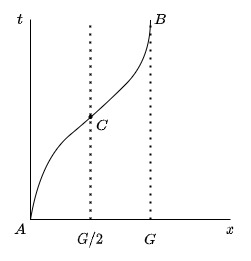
\includegraphics[width=0.50\textwidth]{images/galactic_center_minkowski.jpg}
  \end{center}
  \caption{The worldline of the traveller is composed of two arcs of hyperbola
  $AC$ and $CB$. $G$ indicates the distance to the galactic center.}
  \label{galactic_center}
\end{figure}

\[
  \begin{align}
    t &= g^{-1} \sinh g \tau \\
    x &= g^{-1} \cosh g \tau
  \end{align}
\]
\[
  \tau = g^{-1}\sinh^{-1} gt
\]
\[
  \begin{align}
    x &= g^{-1} \cosh(\sinh^{-1} gt) \\
      &= g^{-1} \sqrt{1 + (gt)^2}
  \end{align}
\]
\[
  \begin{align}
    dx &= \frac{gt}{\sqrt{1 + (gt)^2}} dt
  \end{align}
\]
\[
  \begin{align}
    dt' &= \sqrt{dt^2 - dx^2} \\
        &= \sqrt{dt^2 - \Big(\frac{gt}{\sqrt{1 + (gt)^2} }\Big)^2dt^2}\\
        &= \sqrt{1 - \frac{(gt)^2}{1 + (gt)^2}}dt\\
        &= \sqrt{\frac{1 + (gt)^2 - (gt)^2}{1 + (gt)^2 }}dt\\
        &= \frac{1}{\sqrt{1 + (gt)^2 }}dt\\
  \end{align}
\]
Using an integral table:
\[
  t' = \int \frac{dt}{\sqrt{1+(gt)^2} } = \ln (gt + \sqrt{1+(gt)^2}) = \sinh^{-1}(gt)
\]
\end{enumerate}
\chapter{Incompatibility of Gravity and Special Relativity}
\chapter{Differential Geometry: An Overview}
\chapter{Differential Topology}
\begin{enumerate}
  \item \textbf{COMPONENT MANIPULATIONS}

  \textbf{Derive equations:}
  \[
    u^\alpha = \langle \boldsymbol{\omega}^\alpha \boldsymbol{u} \rangle
  \]
  Consider:
  \[
    \begin{align}
      \langle \boldsymbol{\omega}^\alpha, \boldsymbol{u} \rangle &= u^\beta \langle \boldsymbol{\omega}^\alpha, \boldsymbol{e}_\beta \rangle \\
                                                                 &= u^\beta \delta^\alpha_\beta \\
                                                                 &= u^\alpha
    \end{align}
  \]
  \[
    \sigma_\beta = \langle \boldsymbol{\sigma}, \boldsymbol{e}_\beta \rangle
  \]
  \[
    \begin{align}
      \langle \boldsymbol{\sigma}, \boldsymbol{e}_\beta \rangle &= \sigma_\alpha \langle \boldsymbol{\omega}^\alpha, \boldsymbol{e_\beta} \rangle \\
      &= \sigma_\alpha \delta^\alpha_\beta \\
      &= \sigma_\beta
    \end{align}
  \]
  \[
    \langle \boldsymbol{\sigma}, \boldsymbol{u} \rangle = \sigma_\alpha u^\alpha
  \]
  \[
    \begin{align}
      \langle \boldsymbol{\sigma}, \boldsymbol{u} \rangle &= \sigma_\alpha u^\beta \langle \boldsymbol{\omega}^\alpha, \boldsymbol{e}_\beta \rangle\\
                                                          &= \sigma_\alpha u^\beta \delta^\alpha_\beta \\
                                                          &= \sigma_\beta u^\beta 

    \end{align}
  \]
\end{enumerate}
\end{document}
